\documentclass[a4paper]{article}

\usepackage{a4wide}
\usepackage{algorithm}
\usepackage{algpseudocode}
\usepackage{amsmath}
\usepackage{amssymb}
\usepackage{caratula}
\usepackage{comment}
\usepackage[utf8]{inputenc}
\usepackage{tikz}


\usetikzlibrary{arrows.meta}

\usepackage{fancyhdr}
\pagestyle{fancy}

%\renewcommand{\chaptermark}[1]{\markboth{#1}{}}
\renewcommand{\sectionmark}[1]{\markright{\thesection\ - #1}}

\fancyhf{}

\fancyhead[LO]{Sección \rightmark} % \thesection\ 
\fancyfoot[LO]{\small{Trabajo Práctico 1}}
\fancyfoot[RO]{\thepage}
\renewcommand{\headrulewidth}{0.5pt}
\renewcommand{\footrulewidth}{0.5pt}
\setlength{\hoffset}{-0.25in}
\setlength{\textwidth}{16cm}
%\setlength{\hoffset}{-1.1cm}
%\setlength{\textwidth}{16cm}
\setlength{\headsep}{0.5cm}
\setlength{\textheight}{25cm}
\setlength{\voffset}{-0.4in}
\setlength{\headwidth}{\textwidth}
\setlength{\headheight}{13.1pt}

\renewcommand{\baselinestretch}{1.1}  % line spacing

\setboolean{showKeywords}{false}

\begin{document}

\materia{Algoritmos y Estructuras de Datos III}
\submateria{Primer Cuatrimestre de 2017}
\titulo{Recuperatorio de Trabajo Práctico I}
\subtitulo{Indiana Jones en búsqueda de la complejidad esperada}
%\grupo{Grupo }
\integrante{Arroyo, Luis Alberto}{913/13}{luis.arroyo.90@gmail.com} % obligatorio 

\maketitle

\newpage

\thispagestyle{empty}
\vfill

\thispagestyle{empty}
\vspace{3cm}
\tableofcontents

\newpage

\section{Introducción}

En este informe, vamos a analizar la resolución de un mismo problema, en este caso el de encontrar dos subsecuencias, una creciente y una decreciente dentro de una secuencia de numeros, de manera tal
que ambas secuencias tentas pintadas la mayor cantidad de números posible.

Para ello resolveremos este problema de tres formas distintas:
La primera será resuelta por medio de Backtracking,en la segunda se le agregará una poda al mismo algoritmo del ejercicio 1 y por ultimo se explicará un algoritmo de programacion dinámica.

Cada ejercicio presentará con una introducción explicación, hipotesis de complejidad, resolución y conclusion.


\newpage

\section{Problema I: Bactracking}

%El pseudocodigo de enviar tipos esta muy hablado (lo cual no tengo idea si siquiera es posible escribirlo de otra forma)
%En el primer grafico de tiempos, no se dice en que unidad de tiempo esta medido. En el segundo grafico tmb
%Falta explicar los experimentos y decir que sucede en ellos
%Faltan los test para corroborar correctitud del algoritmo (ejemplos de resultados del algoritmo para mostrar que funcionan)
\subsection{Introducción}
Vamos a utilizar un algoritmo de backtraking que, en el peor caso debería decorrer todas las ramas del arbol de soluciones. Dicha complegidad será exponencial debido a que cada
valor  tiene tres posibilidades, ser pintado de rojo, azul o no ser pintado.


\begin{tikzpicture}[sibling distance=10em,
  every node/.style = {shape=rectangle, rounded corners,
    draw, align=center,
    top color=white, bottom color=white}]]
  \node {v1,v2,v3}
    child { node {v1, Rojo}
        child{ node {v2, Rojo}
            child{ node {v3, Rojo}}
            child{ node {v3, Azul}}
            child{ node {v3, SC}}}
        child{ node {v2, Azul}}
        child{ node {v2, SC}}}
    child { node {v1, Azul}}
    child { node {v1, SC}
 };
\end{tikzpicture}
\vspace*{5mm}

Cada yba de las hojas ultimas hojas del arbol son las posibles soluciones. En particular este arbol al tener 3 hijos va a tener 3 a la n soluciones.
\vspace*{5mm}


\subsection{Resolución del problema y representación}
Para resolver este problema con backtracing, se iterará en toda la lista substecuencias de tamaño 1 hasta el tamaño total de la secuencia
buscando la combinación maxima de elementos rojos y azules pintados. Para realizarlo presentaré el siguiente algoritmo.


Dicho  algoritmo tine como representacion dos vectores uno de enteros no negativos llamado elementos, otro de booleanos llamado validar y dos pilas una roja y otra azul con las siguientes caracteristicas:
\begin{itemize}
    \item Los elementos de las pilas son las posiciones de los elementos de las secuencias.
    \item Una pila es estrictamente creciente y la otra decreciente.
    \item Las pilas son disyuntas entre si.
    \item Todos los elementos de las pilas estan en elementos.
    \item Cuando un elemento ingresa a una pila, se asigna false a la posición de validar del elemento que ingreso.
    \item el vector validad me permite saber que elemento puedo agregar a la pila.
\end{itemize}

\subsection{Algoritmo}


El algoritmo consta de las siguientes funciones:

La función rojos se encarga de encontrar la subsecuencia maxima entre 0 e i, luego la funcion azules hace lo mismo pero siempre entre 0 y n
cada vez que un elemento es agregado a rojos o a azules, el vector validar se establece en falso para dicha posicion.



Podemos observar por medio de los ejemplos que no hay una forma clara de resolverlo sin utilizar este método: minimizar el tiempo de las idas sirve en el ejemplo 1 pero no en el ejemplo 2.
Minimizar el tiempo de las vueltas funciona para el ejemplo 2 pero no para el 1.
También podemos notar que no hay un principio de optimalidad claro: el estado 3 de menor tiempo se consigue siguiendo los pasos del ejemplo 1, pero el ejemplo 2 requiere otro estado 3 para dar el resultado óptimo.

\vspace*{5mm}

Nuestra solución primero verifica que no haya más caníbales que arqueólogos, de haber algún arqueólogo.
En ese caso, ya en el estado inicial los caníbales se los comerían.

Luego se arma el puente que cuenta con 2 objetos ``orilla'' y métodos para mover arqueólogos y caníbales de una orilla a la otra. Las orillas contienen una lista de arqueólogos y una de caníbales.

\begin{algorithm}[H]
\caption{resolver}
\begin{algorithmic}[1]
  \Procedure{resolver}{\texttt{List<Long>} arq, \texttt{List<Long>} can} $\to $ \texttt{long}
    \State \textbf{//Verifico si no hay solución.}

    \If {arq.size() $<$ can.size() $\land$ arq.size() $>$ 0}
		\State	return -1;
	\EndIf

	\State	tTotal $\gets$ $\infty$;

	\State	Orilla origen $\gets$ new Orilla(arq, can);	\State \textbf{//orilla con todos al comienzo}

	\State	Orilla destino $\gets$ new Orilla();
	\State \textbf{	//orilla destino}

	\State	Puente puente $\gets$ new Puente(origen, destino)

	\State	estados $\gets$ new ArbolEstados(arq.size(),can.size());

	\State	res $\gets$ Ida(puente, 0);

	\State return res

 \EndProcedure
\end{algorithmic}
\underline{Complejidad:} $\mathcal{O}(N+M) + \mathcal{O}(ida)$

\vspace*{5mm}
\end{algorithm}

Como recorrer una rama del árbol de backtracking es equivalente a moverse de un estado a otro inmediato (enviando una sola vez gente por el puente), y siendo que se pueden tanto enviar como recibir hasta 2 personas, los estados pueden repetirse.

Para eso creamos un árbol de estados, el cual tiene N+1 nodos representando cada uno la cantidad de arqueólogos que tiene una orilla, y cada uno de estos nodos tiene M+1 nodos hijos, representando la cantidad de can\'ibales en la misma orilla.
Cada nodo de can\'ibales posee una lista con todos los estados donde la orilla guardada tiene la cantidad de arqueólogos y caníbales correspondientes a la rama.
\\

La estructura de \'arbol es muy \'util en \'esta situaci\'on ya que permite conseguir la lista de los estados con la cantidad de arque\'ologos y can\'ibales del estado buscado, acotando la b\'usqueda significativamente.

\vspace*{5mm}
\begin{center}
\begin{tikzpicture}[level/.style={sibling distance=60mm/#1}][H]
\node [rectangle, rounded corners, draw] (z){Raiz}
  child {node [circle,draw] (a) {0}
    child {node [circle,draw] (b) {0}
        child {node [rectangle, rounded corners, draw] (c) {$Estados_{0,0}$}}
    }
    child {node [circle,draw] (d) {M}
        child {node [rectangle, rounded corners, draw] (e) {$Estados_{0,M}$}}
    }
  }
  child {node [circle,draw] (f) {N}
    child {node [circle,draw] (g) {0}
        child {node [rectangle, rounded corners, draw] (h) {$Estados_{N,0}$}}
    }
child {node [circle,draw] (l) {M}
    child {node [rectangle, rounded corners, draw] (j) {$Estados_{N,M}$}
        child [grow=right] {node (q) {$=$} edge from parent[draw=none]
            child [grow=right] {node (r) {Listas de Estados} edge from parent[draw=none]
                child [grow=up] {node (s) {Caníbales} edge from parent[draw=none]
                    child [grow=up] {node (t) {Arqueólogos} edge from parent[draw=none]
                        child [grow=up] {node (u) {Raiz} edge from parent[draw=none]}}
                    }
                }
            }
        }
    }
};
\path (a) -- (f) node [midway] {...};
\path (b) -- (d) node [midway] {...};
\path (g) -- (l) node [midway] {...};
\end{tikzpicture}
\end{center}
\newpage
\vspace*{5mm}
Verificar el estado es equivalente a recorrer los N+1 nodos representando la cantidad de arqueólogos y luego los M+1 nodos de los caníbales hasta dar con la lista de estados con esas cantidades.
Luego, hay que recorrer una lista de estados que potencialmente tiene todas las combinaciones de estados sin repetici\'on, que a lo sumo son
\[
\binom{N+M}{(N+M)/2}
\]

Los estados se guardan y verifican antes de enviar personas por el puente, en las funciones \textit{ida()} y \textit{vuelta()}.

Para pasar de un estado a otro debemos verificar qué acciones se pueden tomar. Para ello armamos 5 funciones que prueban las posibles combinaciones para enviar gente por el puente (1 o 2 arqueólogos, 1 o 2 caníbales y uno de cada) llamadas \textbf{prueboEnviar\textit{personas}} donde \textit{personas} son las combinaciones antes descritas. Cada una de \'estas utiliza el m\'etodo correspondiente de la clase Puente.
\\

Mostraremos como creamos todas las ramas donde enviamos 2 arqueólogos. Primero, el m\'etodo de la clase Puente correspondiente es enviarArq(long,long):

\begin{algorithm}[H]
\caption{enviarArq}
\begin{algorithmic}[1]
    \Procedure{enviarArq}{long i, long j} $\to $ \texttt{long}
        \If {$orilla1.arqSize() < 2 \lor (orilla1.dif() < 2 \land orilla1.arqSize() > 2) \lor orilla2.dif() < -2$ }
            \State	return -1;
        \EndIf
		\State tiempo $\leftarrow$ orilla1.getArq(max(i,j));
		\State orilla2.addArq(tiempo);
		\State tiempo2 $\leftarrow$ orilla1.getArq(min(i,j));
		\State orilla2.addArq(tiempo2);
	    \State \State return $Math.max(tiempo, tiempo2)$
    \EndProcedure
\end{algorithmic}
\underline{Complejidad:}
$\mathcal{O}(N) + \mathcal{O}(1) + \mathcal{O}(N) + \mathcal{O}(1) = \mathcal{O}(N)$

\vspace*{5mm}
\underline{Justificación:} Borramos los arque\'ologos de la Orilla origen y los agregamos a la Orilla destino. getArq() cuesta $\mathcal{O}(N)$ y addArq() cuesta $\mathcal{O}(1)$. Luego devolvemos el m\'aximo de los tiempos, que es lo que tardan ambos en cruzar el puente.


\underline{Observaciones:} Se pueden enviar todas las combinaciones de 2 arque\'ologos o ninguna. En el segundo caso, devuelve "-1" en $\mathcal{O}(1)$
\end{algorithm}

La funcion \textit{dif()} devuelve la cantidad de can\'ibales de una orilla menos la cantidad de arque\'ologos de la misma. El \textbf{if} verifica si hay 2 arque\'ologos para enviar, y que si \'estos se env\'ian no queden m\'as can\'ibales que arque\'ologos en alguna de las 2 orillas que tenga alg\'un arque\'ologo.

\begin{algorithm}[H]
\caption{prueboEnviar2Arqueologos}
\begin{algorithmic}[1]
  \Procedure{prueboEnviar2Arqueologos}{Puente p, long tParcial, long tVueltaMin,  boolean ida} $\to $ \texttt{long}
    \For {$i = 0; i < N{-}1; i{+}{+}$}
        \For {$j = i{+}1; j < N; j{+}{+}$}
            \State $q \leftarrow p$
        	\State $t \leftarrow q.enviarArq(i,j)$;
        	\If {$t < 0$}
        		\State	return -1;
        	\EndIf
        	\State \textit{//Comparo el tiempo hasta este estado con el tiempo total, para podar}
        	\If {$tParcial + t < tTotal$}
        		\State	tVuelta $\leftarrow$ vuelta(p,tParcial+t)
        		\If {$tVuelta \geq 0 \land (t + tVuelta) < tVueltaMin$}
        		    \State \textit{//Me quedo con el mejor tiempo desde \'este estado hasta el estado final}
            		\State	tVueltaMin $\leftarrow$ t + tVuelta
            		\State  tTotal $\leftarrow$ (tParcial + tVueltaMin)
            	\EndIf
        	\EndIf
    	\EndFor
	\EndFor
	\State \State return $tVueltaMin$
 \EndProcedure
\end{algorithmic}
\underline{Complejidad:}
$\mathcal{O}(N^2) * (\mathcal{O}(enviarArq()) + \mathcal{O}(Ida()))$= $\mathcal{O}(N^3) + \mathcal{O}(N^2)*\mathcal{O}(Ida())\Rightarrow \mathcal{O}(N^3)$+ recursión.

\vspace*{5mm}
\underline{Justificación:} Iteramos sobre todas las combinaciones de 2 arqueólogos posibles, y los movemos de una orilla a la otra.
Moverlo cuesta lo mismo que recorrer la lista de arqueólogos y eliminar el buscado, que es $\mathcal{O}(N)$.
Luego, llamamos a la función ida (o vuelta, que tiene la misma complejidad)
\end{algorithm}

\underline{Observaciones:}
\begin{itemize}
    \item De aqu\'i en m\'as omitiremos el \textit{+recursi\'on} en los c\'alculos de complejidad dado que luego calcularemos la complejidad total del algoritmo en base al costo de los nodos sin la recursi\'on.
    \item enviarArq(i,j) tiene la misma complejidad que enviarArq(i), vuelveArq(i,j) y vuelveArq(i). Idem para las funciones sobre caníbales, que todas son del orden $\mathcal{O}(M^3)$. enviarAmbos() y vuelvenAmbos() son del orden $\mathcal{O}(N*M * (N+M))$. Todas las complejidades podrían escribirse como $\mathcal{O}({max(N,M)}^3)$ o $\mathcal{O}({(N + M)}^3)$
\end{itemize}
\begin{comment}
Creemos que calcular el tiempo de enviar los arqueólogos a la otra orilla se podría reducir a $\mathcal{O}(1)$ con un iterador con lo que el algoritmo sería $\mathcal{O}(N^2)$ + recursión. En nuestro intento el código no andaba y decidimos dejarlo como se encuentra en la versión final.
\end{comment}

\textbf{tParcial}: Siendo que ésta función se llama en el $Estado_i$, tParcial acumula el tiempo desde $Estado_0$ hasta $Estado_{i-1}$.

\textbf{tVueltaMin}: Con ésta variable se devolverá el tiempo desde $Estado_i$ hasta $Estado_{final}$.

\textbf{tTotal}: Es el tiempo de la mejor solución encontrada.

\textbf{ida}: Indica si el método es llamado desde \textit{ida()} o \textit{vuelta()}. En éste caso, escribimos el pseudocódigo como si fuera llamado desde \textit{ida()}

\vspace*{5mm}

Por último, los métodos principales que representan los nodos del backtracking son \textit{ida()} y \textit{vuelta()}. La diferencia principal en ambos es que \textit{vuelta()} debe verificar al comenzar si se ha llegado al estado final, pues de ser así no hay que enviar a nadie de regreso a la orilla de origen.

\begin{algorithm}[H]
\caption{Ida}
\begin{algorithmic}[1]
  \Procedure{Ida}{Puente p, long tParcial} $\to $ \texttt{long}
  \State Ordeno la orilla origen (para comparar correctamente los estados)
  \State Verifico que éste estado no haya sido alcanzado previamente en un tiempo menor \\ con checkEstado().
  \State
  \State Pruebo todas las formas de enviar 2 arqueólogos.
  \State Pruebo todas las formas de enviar 2 caníbales.
  \State Pruebo todas las formas de enviar 1 arqueólogo y 1 caníbal.
  \State Pruebo todas las formas de enviar 1 arqueólogo.
  \State Pruebo todas las formas de enviar 1 caníbal.
  \State
  \State Si ninguna de las anteriores fue posible o tardaron más que una solución previa, devuelvo -1.
  \State De otra forma, devuelvo el tiempo que cuesta la mejor solución a partir del estado actual.
 \EndProcedure
\end{algorithmic}
\underline{Complejidad:}
 $\mathcal{O}(Sort()) + \mathcal{O}(checkEstado()) + \mathcal{O}(5*pruebo[...]())$ = $\mathcal{O}((N+M)*log_2(N+M)) + \mathcal{O}(\binom{N+M}{(N+M)/2}) + \mathcal{O}(5*max(N,M)^3) = \mathcal{O}(\binom{N+M}{(N+M)/2}) = \mathcal{O}((N+M)!)$

 \vspace*{5mm}
 \underline{Justificación:}
 Ordenamos con Collections.sort() que está documentado como $\mathcal{O}((N+M)*log_2(N+M))$. El tiempo de checkEstado() se justificó en el dibujo del árbol de estados. Luego, si el estado no fue previamente visitado en un tiempo menor, ejecutamos 5 funciones con el mismo tiempo que prueboEnviar2Arqueologos().

\end{algorithm}
\begin{comment}
\underline{Observaciones:}
 $\binom{N+M}{(N+M)/2}$ es $\mathcal{O}((N+M)!)$ para el caso general, con lo que podría ser necesario mejorar como se guardan los estados. Una mejora básica sería guardar únicamente las orillas con menos personas, reduciendo el peor caso de  $\binom{N+M}{(N+M)/2}$ a $\binom{(N+M)/2}{(N+M)/4}$. Otra forma sería agregar más nodos intermedios al árbol de estados, como la suma de los tiempos de los arqueólogos y la suma de los tiempos de los caníbales. De esa forma subdividiríamos las listas en más nodos que sólo costarían N y M respectivamente (y podrían ser valores que se guarden en memoria con un índice, consiguiéndolos en $\mathcal{O}(1)$). La complejidad temporal sigue siendo la misma (en el peor caso todos tienen los mismos tiempos), pero mejoraría rápidamente si hay pocas repeticiones. En el caso ideal los tiempos de cada arqueólogo/caníbal son distintos entre sí, con lo que cada estado estaría unívocamente representado por la suma de los tiempos de unos y otros, y encontrarlos podría ser $\mathcal{O}(1)$ si logro ubicarlas con índices (con lo que la mejora temporal tampoco está asegurada). El costo de memoria empeoraría inversamente proporcional a como mejora el costo temporal con éste método.
\end{comment}

En una versión anterior de nuestro código, el método \textit{vuelta()} evaluaba los métodos para enviar personas a la orilla origen en el mismo orden que \textit{ida()}.
En un análisis posterior notamos que salvo un caso (3 arqueólogos y 3 caníbales) los únicos movimientos que se utilizaban en la solución óptima eran de enviar 2 personas a la orilla destino y retornar una.

Si bien no pudimos probar cuánto se utilizan las opciones de enviar una persona o de retornar 2, mostraremos en la sección de experimentación la diferencia de tiempos entre ése código y el de la versión final, donde \textit{vuelta()} primero evalúa retornar una sola persona a la orilla origen.

%\newpage
\subsection{Correctitud}

\textbf{Terminación:} El algoritmo termina, dado que en el peor caso revisa todos los estados (cantidad finita). Un mismo estado sólo es analizado nuevamente siempre que se llegue en un tiempo menor que todas las veces anteriores, con lo que sólo pueden ser visitados una cantidad finita de veces al tener una cantidad finita de arque\'ologos y can\'ibales, todos con tiempos positivos.
Recorremos de a una rama a la vez hasta el final. Una vez que llegamos al final de la rama, retrocedemos un estado en la rama, llamémoslo E, y vemos si existe otra rama no analizada que se pueda bifurcar a partir de este estado. Si existe, la analizamos de la misma forma. Cuando terminamos de analizar la rama, al ir retrocediendo terminamos en el mismo estado E. Luego verificamos si quedan más ramas para repetir el proceso, o si no hay más ramas, retrocedemos en la rama hasta un estado E' y repetimos el proceso hasta analizar todos los estados, llegando hasta la raíz del árbol que se forma. Cuando desde la raíz no hay más bifurcaciones sin analizar, el algoritmo termina porque analizó todos los estados que podrían ser soluciones. Si hay estados que fueron podados, fue porque sabemos que no eran soluciones deseadas:

Las cotas de tiempos podan estados que se acceden en un tiempo mayor a una solución anteriormente encontrada.
Por lo tanto, no evita que encontremos la solución óptima.
Tampoco las podas que no nos permiten movernos a estados inválidos, pues la solución óptima requiere que todos los pasos sean válidos.
 \\

\textbf{Reviso todas los estados alcanzables desde el estado inicial:}
\\
Quiero ver que puedo acceder a todo estado $E_i$ que sea válido y alcanzable desde el estado inicial por una cantidad finita de pasos.
\\

\textbf{P(i): } Se accede al estado $E_i$ si éste es válido y existe al menos un estado $E_{i-1}$ válido y alcanzable que difiera en una operación válida (teniendo en cuenta la ubicación de la linterna y la distribución de arqueólogos y caníbales). A partir de este estado $E_{i-1}$ aplicamos un movimiento permitido para poder acceder a este estado $E_i$.
\\

\textbf{Caso base: } El estado $E_0$ se accede dado que es el estado inicial, en el cual todos los arqueólogos y caníbales están del mismo lado y poseen la linterna. Dado que un estado inicial inválido no tiene sentido para el problema, asumiremos que siempre es válido.
\\

%Los estados $E_1$ se acceden por medio de los pasos válidos a partir del único caso $E_0$ (enviando 1 o 2 personas de origen a destino, en cualquier combinación válida)
%\\

\textbf{Paso inductivo: P(i) $\rightarrow$ P(i+1): }  Tengo el conjunto de estados $E_i$. Son válidos y alcanzables por el algoritmo por la HI. A partir de aquí tenemos varias posibilidades:

\begin{itemize}
    \item Si el conjunto de los estados $E_i$ es vacío, entonces el estado $E_{i+1}$ no es un estado válido, dado que no hay una combinación de movimientos válidos a partir del estado inicial con la cual llegar a este estado. Como no existe un estado anterior válidamente alcanzable, la propiedad P(i+1) resulta ser verdadera.

    \item Si el conjunto de estados no es vacío, entonces para todos los estados $E_{i}$ puedo realizar alguna de las operaciones para mover algún arqueólogo o caníbal.
    \begin{itemize}
    \item Si ningún estado puede realizar alguna operación que sea válida (es decir, que puedan trasladarse personas con la linterna y que los caníbales no devoren a alg\'un arqueólogos), entonces el estado $E_{i+1}$ no es un estado para el cual exista alguna secuencia de movimientos válidos de arqueólogos y/o caníbales para alcanzarlo. Como no se cumple esta propiedad, P(i+1) resulta ser verdadera.

    \item Nombremos a la operación valida desde el estado $E_{i}$ para llegar a $E_{i+1}$ como $Op_{i+1}$. Llamemos también $S_i$ a la secuencia de operaciones válidas que se utiliza para llegar al estado $E_{i}$, la cual existe por HI. Si agregamos $Op_{i+1}$ al final de la secuencia $S_i$, obtenemos una secuencia de operaciones válidas desde el estado inicial hasta el estado $E_{i+1}$ por la cual accederlo. De esta forma la propiedad P(i+1) resulta ser verdadera.
    \end{itemize}
\end{itemize}


De esta forma probamos que alcanzamos a todos los estados. Por ende, si existe una solución válida la encontramos. Más aún, como podamos por tiempos quedándonos siempre la mejor solución que encontramos, siempre vamos a visitar el estado final que se consigue en el menor tiempo.

Para el caso que no exista solución, inicializamos ciertas variables en -1 para indicar que no hemos conseguido una solución. Si al final del algoritmo éstas variables no cambiaron, sabemos que no hay solución.
\subsection{Complejidad del algoritmo}
\subsubsection{Complejidad demostrada}
Cada estado tiene $\mathcal{O}{(N+M)}^2$ estados hijo (ignorando podas).

Como cada rama podr\'ia visitar cada uno de los estados, la altura máxima es $(N+M)!$, ignorando que siempre intentamos acercarnos a la solución en cada paso probando enviar 2 personas y devolver 1.

Podemos conseguir la cantidad de nodos de un árbol m-esimo de altura h con la fórmula

\[
\sum_{i=0}^{h}{m}^{i} = \frac{1 - m^{h+1}}{1 - m}
\]

La igualdad es válida por ser una serie geométrica.

Ésto hace que la cantidad de nodos del árbol de backtracking sea
\[
\sum_{i=0}^{(N+M)!}{(N+M)}^{2i} \Rightarrow \mathcal{O}({(N+M)}^{2(N+M)! +2 })\Rightarrow \mathcal{O}({(N+M)}^{(N+M)!})
\]

Cada nodo cuesta $\mathcal{O}((N+M)!)$ como fue demostrado en el pseudocódigo del algoritmo \textit{ida()}

\vspace*{5mm}
\textbf{Resultado:}
\[
\mathcal{O}({(N+M)}^{(N+M)!} * (N+M)!)
\]


\subsubsection{Complejidad tomando en cuenta las podas}
La complejidad teniendo en cuenta que la gran mayoría de los movimientos son de enviar 2 personas de ida y 1 de vuelta, con lo que la cantidad de estados que se recorrerán por rama (altura del árbol) es aproximadamente N+M:
\[
\mathcal{O}({(N+M)}^{(N+M)} * (N+M)!)
\]

%\newpage
\subsection{Experimentación}

Primero generamos una serie de tests para verificar el algoritmo.
Éstos tests fueron creados a mano intentando cubrir la mayor cantidad de casos interesantes. El más destacable es el caso de 3 arqueólogos y 3 caníbales, que requiere que \textit{vuelta()} envíe a la orilla origen 2 personas.
También probamos quitar en \textit{resolver()} la verificacion de if ($N < M \land N > 0$) then return -1 y probar con esos casos. Como era de esperar éstos devolvieron "-1".

\vspace*{5mm}
Luego armamos un generador de casos aleatorios para graficar los tiempos del algoritmo (en nanosegundos).

El generador recorre, para cada N+M, todas las combinaciones de N y M (N $\geq$ M). Para cada uno de éstas combinaciones se crean 10 problemas que se ejecutan 10000 veces para que la cache de la jvm no influya, y luego se toma el tiempo promedio de las siguientes 10000 ejecuciones. Para un mismo N+M se promedian todos los promedios y ése es el valor que se grafica.
\\

En el primer gráfico se muestra el algoritmo donde \textit{ida()} y \textit{vuelta()} evalúan enviar primero 2 personas a la otra orilla. Ésta versión del algoritmo está claramente acotado por $\mathcal{O}({(N+M)}^{(N+M)} * (N+M)!)$. Aún más exacto es acotar el algoritmo por $\mathcal{O}({(N+M)}^{(N+M)})$. \'Esta cota sale de los experimentos, mostrando que nuestras podas mejoran mucho el algoritmo respecto al peor caso demostrado (sin podas).


\begin{figure}[H]
    \centering
    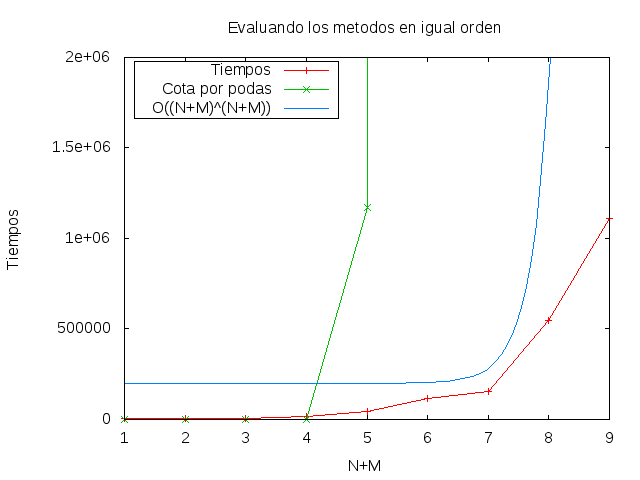
\includegraphics[width=10cm]{./imagenes/tiemposEj1Igual.png}
    \caption{Tiempos evaluando en el mismo orden la forma de enviar personas a la otra orilla}
    %\label{fig:my_label}
\end{figure}

\newpage

En el segundo gráfico podemos observar la diferencia de desempeño entre el algoritmo utilizado en el gráfico anterior, y la versión final del mismo donde la única diferencia es que \textbf{vuelta()} primero evalúa enviar 1 persona a la orilla origen.


\begin{figure}[H]
    \centering
    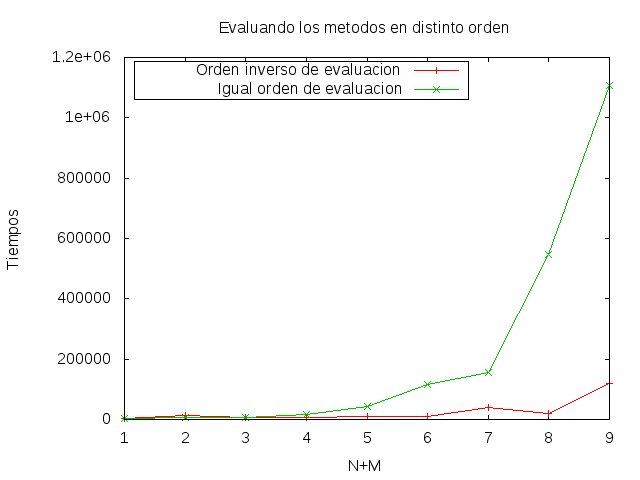
\includegraphics[width=10cm]{./imagenes/tiemposEj1Cambiados.png}
    \caption{Diferencia de tiempos entre evaluar los métodos de la misma forma o discriminar entre ida() y vuelta()}
    %\label{fig:my_label}
\end{figure}

Para mayor detalle, agregamos gráficos fijando N y variando M y viceversa, y los comparamos con los promedios antes tomados.

\begin{figure}[H]
    \centering
    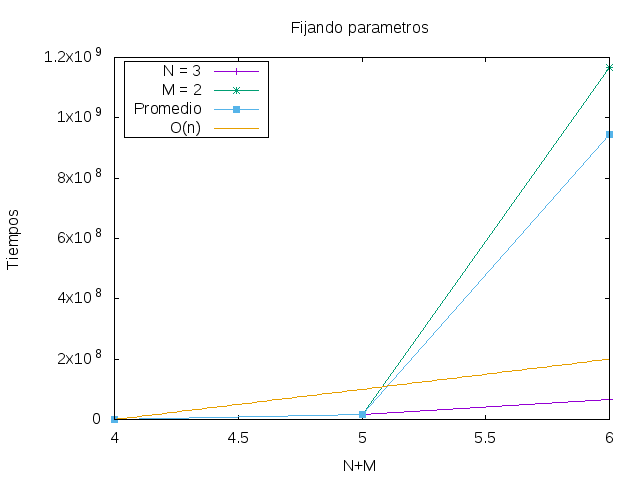
\includegraphics[width=10cm]{./imagenes/fijos.png}
    \caption{Diferencia para un mismo N y M respecto al promedio de todas las combinaciones válidas}
    %\label{fig:my_label}
\end{figure}

Podemos ver como para un mismo N+M, se ve m\'as influyente la cantidad de arque\'ologos que la cantidad de can\'ibales. Entendemos que esto ocurre porque cuando N y M son iguales, las operaciones v\'alidas para los estados son menos que las operaciones v\'alidas cuando N es mayor a M. Y como devolvemos en $\mathcal{O}(1)$ que una operaci\'on no es v\'alida, la curva de N=3 es mucho menor que la curva de M=2


\newpage

\section{Problema II: Problemas en el camino}

\subsection{Introducción}

%Explicación informal
En este ejercicio, el grupo de arqueólogos necesita abrir una puerta cerrada con llave. En la misma habitación hay una balanza con dos platillos, y sobre uno de los platillos se encuentra la llave de la puerta. Al sacar la llave de la balanza, ésta cambia su equilibrio, la puerta se cierra y las paredes comienzan a moverse hacia ellos con el fin de aplastarlos. Para frenar las paredes y poder usar la llave, los arqueólogos tienen que volver la balanza a su equilibrio inicial utilizando un conjunto de pesas (ya que necesitan la llave como para volverla a colocar en la balanza), que tienen como peso una potencia de tres (no hay pesas del mismo peso). Para la suerte de los arqueólogos, uno de ellos tiene una balanza digital que les indica el peso de la llave que deben restablecer.

%Conectar la explicación informal con la formal
Dicho de forma más formal, dado el peso de la llave, se debe restablecer la balanza, de forma tal que la sumatoria de los pesos que se coloquen en el platillo donde estaba la llave, restada a la sumatoria de los pesos que se coloquen en el otro platillo, sea equivalente al peso de la llave.



\subsection{Resolución del problema}

Como los pesos en ambos platillos son sumatorias de potencias de 3, decidimos representar el peso de la llave como un número escrito en base 3. Este número nos dice que el valor $a_i$ del número, siendo $i$ la posición del valor comenzando a contar desde el valor menos significativo, es la constante que multiplica a la potencia $3^i$, el cual puede ser $0,\ 1\ o\ 2$. Estas constantes nos van a servir para saber qué pesas tenemos que utilizar en qué balanza. Por cada dígito de la representación del peso de la llave en base 3 tenemos que tomar una decisión según su valor. Entonces tenemos 3 casos distintos:

\begin{itemize}
    \item \textbf{$a_i = 0$: } 
        Este caso indica que no tenemos que poner ninguna pesa en ningún platillo. Como esta potencia de 3 no esta incluida en la sumatoria de potencias de 3 que representa al peso de la llave, no tenemos que agregarla a la balanza.
        
    \item \textbf{$a_i = 1$: } 
        Este caso indica que tenemos que poner la pesa de peso $3^i$ en el platillo donde se encontraba la llave. Esto se debe a que la potencia $3^i$ se encuentra en la sumatoria de potencias de 3 que representa al peso de la llave. 
    
    \item \textbf{$a_i = 2$: } 
        Este caso indica que deberíamos agregar peso para tratar de compensar la sumatoria, pero como solo tenemos un peso de cada potencia de 3, no podemos agregar 2 pesos en el platillo en que estaba la llave. Por eso es que agregamos el peso $3^i$ en el otro platillo y sumamos el valor $3^i$ representado en base 3, al peso de la llave representado también en base 3. Esto equivale a sumarle 1 a $a_i$, que quedaría en 0 y se le suma 1 al valor $a_{i+1}$ (incluyendo también que todos los valores siguientes de la representación sean menores a 3).
        
        Sabemos que esto funciona por la siguiente igualdad:
        $3^{i+1} = 3*3^i = 2*3^i + 3^i$.
        En términos de nuestro problema, $2*3^i$ es el valor que nosotros tenemos y no podemos poner el el platillo de la llave. Entonces si le sumamos el término $3^i$ (es decir, ponemos el peso $3^i$ en el otro platillo para aumentar el peso que tenemos que poner en el platillo de la llave), necesitaríamos agregar el peso $3^{i+1}$ al platillo de la llave. 
        
\end{itemize}

Como se puede observar en el último de nuestros casos, para evitar problemas por sumarle 1 al valor $a_{i+1}$, tenemos que analizar este valor luego de analizar todos los valores menos significativos antes para tener los valores posteriores que serán usados efectivamente.

Sabiendo como operar con cada dígito de la representación en base 3 del peso de la llave, procedemos a armar nuestro algoritmo. Éste consiste en iterar sobre cada dígito de la representación, del valor menos significativo hasta el más significativo, y para cada dígito realizar alguno de los 3 casos descriptos previamente. 

Para facilitar los cálculos, cuando ``nos llevamos una'', establecemos una variable booleana como verdadera para indicarnos que en la siguiente iteración tenemos que sumarle 1 al valor.

A continuación incluimos el pseudocódigo del algoritmo:


\subsection{Pseudocódigo}

\begin{algorithm}[h]
\caption{resolver}
\begin{algorithmic}[1]
  \Procedure{resolver}{int peso\_llave} $\to $ \texttt{List<int> platillo\_llave, List<int> platillo\_otro}
  
  
    \State \textbf{//Obtengo la representación en base 3. De valores menos significativos a más significativos.}
	\State \texttt{List<Integer>} key\_weight\_base\_3 $\gets$ toBase3(peso\_llave);	
	
	\State
    \State \textbf{//Booleano para saber si me lleve una o no.}
	\State boolean iTookOne = false;					
	
    \State 
    \For{(int i = 0; i $<$ key\_weight\_base\_3.length; i++)}

		\State \textbf{//Obtengo el valor i de la representación de la base.}
		\State int value = key\_weight\_base\_3.get(i);		
		
		\State 
		\State \textbf{//Si me lleve una antes incremento el valor.}
		\If{(iTookOne)}
		
			\State value++;				
			\State iTookOne = false;
			
		\EndIf
		
		\State 
		\State \textbf{//Agrego las pesas en los platillos correspondientes.}
		\If{(value == 0)}
		
			%\State 
			\State \textbf{//No tengo que poner ninguna pesa.}
			\State 
			
		\ElsIf{(value == 1)}
	
		    %\State 
			\State \textbf{//Tengo que poner la pesa $3^i$ en el lado de la llave.}
			
		    \State platillo\_llave.add($3^i$);
		    \State 
		\ElsIf{(value == 2)}
			
			%\State 
			\State \textbf{//Tengo que poner la pesa $3^i$ en el otro lado y me llevo una para compensar los pesos.}
				
			\State platillo\_otro.add($3^i$);
			\State iTookOne = true;	
			\State 
			
		\Else
			%\State 
			\State \textbf{//No tengo que poner ninguna pesa. Me llevo una para compensar.}
			\State \textbf{//(valor == 3, entonces la consideramos como 0 y me llevo una).}
			
			\State iTookOne = true;
			
		\EndIf	
	
	\EndFor
	
 \EndProcedure
 
\end{algorithmic}
\end{algorithm}



\newpage

\begin{algorithm}
\caption{toBase3}
\begin{algorithmic}[1]
  \Procedure{toBase3}{int peso\_llave} $\to $ \texttt{List<int> base3}
 
		\While{ (peso\_llave $>$ 0) }   		
		
		    \State \textbf{//Obtengo cociente y resto.}
			\State int quotient  = peso\_llave / 3;
			\State int remainder = peso\_llave \% 3;
			
			\State
			\State \textbf{//Actualizo el peso de la llave.}
			\State peso\_llave = quotient;				
			\State
			\State \textbf{//Agrego el valor a la lista resultado.}
			\State base3.add( remainder );		
		
		\EndWhile
		
		\State
		\State return base3;
	
		
		\EndProcedure
 
\end{algorithmic}
 
\end{algorithm}


\subsection{Correctitud}

En esta sección explicaremos por qué el algoritmo funciona. Sabemos que todo número puede representarse como una sumatoria de potencias de una misma base $b$, donde cada potencia puede ser multiplicada por un número menor a $b$. Es decir, para nuestro caso podemos expresar el número $X$ como una sumatoria de potencias de $3$ multiplicadas por un valor  $ 0 \leq a_i \leq 2$: 
\[
\sum_{0}^{\infty}a_i*3^i = X
\]

Si consideramos al término izquierdo de la igualdad como el platillo de la balanza donde se encontraba la llave, y al término derecho de la igualdad como el otro platillo de la balanza, nuestro algoritmo lo que hace es transformar la sumatoria en otra sumatoria de potencias de $3$ pero el valor que multiplica a cada potencia va a ser solamente el valor $0$ o $1$. El valor $X$ de este lado se utiliza simplemente para representar el equilibrio inicial en la balanza y simplificar las cuentas y explicaciones.

Esto lo logramos transformando a las potencias $3^i$ multiplicadas por el valor $2$, en potencias $3^{i+1}$. La transformación se basa en la igualdad $3^{i+1} = 3*3^i = 2*3^i + 3^i$. Usando esta igualdad podemos, escribir al término $2*3^i$ como $3^{i+1}$, siempre y cuando compensemos el término $3^i$ en el otro lado de la igualdad.

Obtenido el término $3^{i+1}$, tenemos 3 casos que analizar: 

\begin{itemize}
    \item \underline{ \textbf{En la sumatoria original, $a_{i+1} = 0$ o $a_{i+1} = 1$: } } En estos casos sumamos el término obtenido en la transformación, y obtenemos que el valor que multiplica a la potencia $3^{i+1}$ ahora es $1$ o $2$. Siendo estos dos los valores que quedan multiplicando a la potencia, podemos proceder a continuar con el algoritmo, el cual manejara a estos valores cuando le toque analizarlos.
    
    \item \underline{ \textbf{En la sumatoria original, $a_{i+1} = 2$: }} En este caso, al sumarle la potencia $3^{i+1}$ obtenida en la transformación, se obtiene el término $3*3^{i+1}$, que es equivalente a $3^{i+2}$. A este nuevo valor lo podemos sumar al término $i+2$ de la sumatoria, teniendo que analizar nuevamente estos 3 casos para ese término.
   
\end{itemize}

Estas últimas operaciones terminan en algún momento, dado que no hay términos infinitos de la sumatoria que tengan $a_{k} = 2$ como valor que multiplica a la potencia $3^k$.

Explicada la razón de porque transformar la sumatoria de la igualdad, nos falta justificar que al terminar de iterar los términos de la sumatoria desde el más chico hasta el más grande, no nos quedan potencias de $3$ con el mismo exponente en ambos lados de la igualdad.

Esto se ve fácilmente de la siguiente forma: cuando estamos iterando el término $i$ de la sumatoria, todos los términos anteriores (que van a ser potencias más chicas que la actual), ya fueron analizadas, y los resultados de estas implicaron que no haya término $3^j$ ($j<i$) en ningún lado de la igualdad, que el término $3^j$ esté del lado izquierdo de la igualdad con $a_j = 1$, o que $3^j$ esté del lado derecho de la igualdad también con $a_j = 1$. Esto nos asegura que al menos hasta la iteración $i$, tenemos a lo sumo solo una potencia $3^i$ entre ambos lados de la igualdad.

Con respecto a los término siguientes a $i$, como mantenemos los valores $a_l$ ($l>i$) iguales a $0,~1~ o~ 2$, siempre van a estar en condiciones de ser resueltos correctamente por iteraciones siguientes del algoritmo.

Una vez que el algoritmo termina, lo que obtenemos es una igualdad de la forma:
\[
\sum_{0}^{\infty}a_i*3^i = X + \sum_{0}^{\infty}b_i*3^i
\]

para las cuales $0 \leq a_i \leq 1$, $0 \leq b_i \leq 1$ y $a_i + b_i \leq 1 $ (es decir que sólo esta la potencia $1*3^i$ en a lo sumo uno de los lados de la igualdad).

Como dijimos al comienzo, el lado izquierdo se corresponde con el platillo donde se encontraba la llave, y el lado derecho de la igualdad se corresponde con el otro platillo. Entonces, por cada término $1*3^i$ del lado izquierdo de la igualdad, tenemos que poner la pesa del mismo valor en el platillo. De forma análoga para el lado derecho, agregamos los valores $1*3^i$ de la sumatoria como pesas del mismo valor en el platillo.

\subsection{Complejidad del algoritmo}

Comenzaremos por la complejidad de la función toBase3(peso). Esta función devuelve la representación en base 3 del número pasado como parámetro y consiste en un ciclo donde las operaciones que se hacen tienen tiempo constante. Estas operaciones son de dividir el número por 3 hasta que el resultado sea 0 y obtener el resto, valor que será un elemento de la representación en base 3 del número. Entonces la complejidad de la función será la cantidad de veces que itere el ciclo. La cantidad de iteraciones que realiza será luego la parte entera superior del logaritmo en base 3 del peso. En la siguiente ecuación buscamos la cantidad de veces que debe iterarse la división para que peso sea menor a 1 (es decir, sea 0):
\[ 
peso/(3^x) < 1 
\] \[
peso < 3^x
\] \[
log_3(peso) < log_3(3^x)
\] \[
log_3(peso) < x
\]

Siendo X la cantidad de veces que dividimos el peso por 3, se ve que X tiene que ser mayor al $log_3$ del peso. Como X es un valor entero, nuestro X será el valor entero superior de $log_3(peso)$.

Como la cantidad de elementos de la lista retornada es uno por cada iteración, la cantidad va a ser también el valor entero superior inmediato a $log_3(peso)$.


Sabiendo esta complejidad, podemos explicar la complejidad de la función resolver(peso). Como se puede observar en el pseudocódigo, todas las operaciones que se realizan son operaciones de tiempo constante. Entonces lo que va a determinar la complejidad del algoritmo es la complejidad de la llamada a la función toBase3(peso) y la cantidad de iteraciones que realiza el ciclo. Este ciclo itera sobre cada uno de los elementos de la representación del número devuelta por la función toBase3(peso). Es decir que va a iterar $log_3(peso) +1$ veces, una por cada dígito de la representación en base 3 de nuestro número, con todas operaciones constantes en cada iteración. 

Sumando las complejidades importantes, tenemos por la llamada a toBase3 la complejidad $log_3(peso)$, y por el ciclo tenemos la misma complejidad.

Luego, la complejidad del algoritmo va a ser $O(log_3(peso))$. Como esta complejidad es menor a $\sqrt{peso}$, cumple con la condición pedida de que la complejidad debe ser menor a $O(\sqrt{peso})$.

\newpage
Mostremos ahora que $O(log_3(x))$ es menor a $O(\sqrt{x})$.

\[
log_3(x) < \sqrt{x}
\] \[
0 < \sqrt{x} - log_3(x)
\]
Derivando $f(x) = \sqrt{x} - log_3(x)$ obtengo :
\[
f'(x) = 1/2\sqrt{x} \ - \ 1/x.ln(3)
\] \[
f'(x) = (1 - 2/\sqrt{x}.ln(3)) \ /2\sqrt{x}
\]

Como puede observarse la derivada es positiva cuando $1 - 2/\sqrt{x}.ln(3)$ lo es. Luego:
\[
1 - 2/\sqrt{x}.ln(3) > 0
\] \[
1 > 2/\sqrt{x}.ln(3)
\] \[
\sqrt{x} > 2/ln(3) \approx 1.82
\]

Y esta desigualdad se cumple cuando $4 \leq x$.
 
De esta forma obtenemos que $f(x) = \sqrt{x} - log_3(x)$ es creciente $\forall x \geq 4$. Calculando $f(4)$:
\[
f(4) = \sqrt{4} - log_3(4) \approx 2 - 1.26185950714291 > 0 \ \forall \ x \geq 4
\]
y como $f(x)$ es creciente, tenemos que 
\[
f(x) > 0 \ \forall x \geq 4
\] \[ 
\sqrt{x} - log_3(x) > 0 \ \forall x \geq 4
\] \[
\sqrt{x} > log_3(x)  \ \forall x \geq 4
\]

Analizando los valores $x = 1,2,3$:

\[
\sqrt{1} = 1 > log_3(1) = 0
\] \[
\sqrt{2} > 1.4 > 0.64 > log_3(2)
\] \[
\sqrt{3} > 1.7 > log_3(3) = 1
\] 

Luego obtuvimos:
\[
\sqrt{x} > log_3(x)  \ \forall x > 0
\]
Y por ende:
\[ 
O(log_3(x)) es menor que O(\sqrt{x})
\]


 

\newpage
\subsection{Experimentación}

Como el único parámetro de entrada del algoritmo es P, como experimentación correremos el programa variando el P en instancias pequeñas e instancias grandes, dado que P puede tomar valores de hasta $10^{15}$.

\begin{figure}[H]
    \centering
    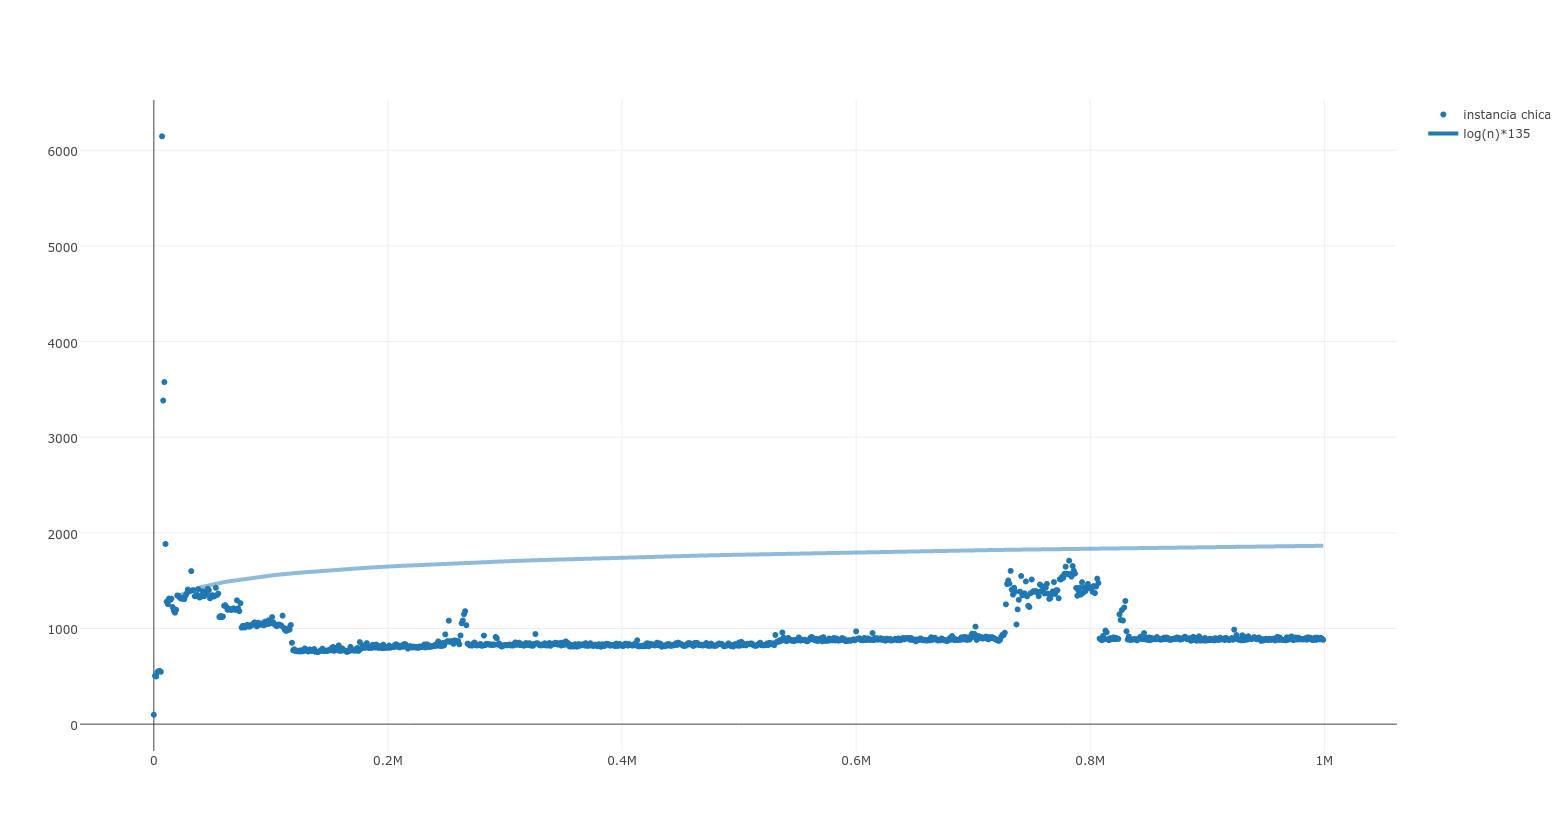
\includegraphics[width=\textwidth]{./imagenes/ej2chico.png}
    %\caption{FCFS con 2 núcleos}
    %\label{fig:my_label}
\end{figure}

Si bien en el gráfico los resultados estan por debado de la función log(P).350, se puede observar que el crecimiento del tiempo de la ejecución de las instancias es muy leve. Esto se debe a que en realidad el algoritmo tiene como complejidad al entero superior próximo de $log_3(x)$. Además, al ser un logaritmo, la instancia más grande da que $log_3(1.000.000)$ $\approx$ 12.6, y para una instancia no tan chica, digamos 100.000, tenemos que $log_3(100.000) \approx 10.5$. Por lo que al ser tan pequeña esta diferencia, ya que los valores enteros de los logaritmos varían entre 11 y 13 (por ser el entero superior mas próximo), la complejidad empírica obtenida pareciera tener un comportamiento constante.
%Para las instancias más chicas se obtuvieron valores anómalos. Estos valores se generaron por operaciones que realiza la JVM de las cuales no tenemos control para evitarlos.
%En el gráfico se puede ver que los tiempos obtenidos se encuentran por debajo de la función $log(P)$. Utilizamos la constante 350 para generar un gráfico en el que se pueda apreciar que ambas curvas tienen un comportamiento de crecimiento de estilo logarítmico. 
\\
Las instancias van de 0 a 1 millón.


\begin{figure}[H]
    \centering
    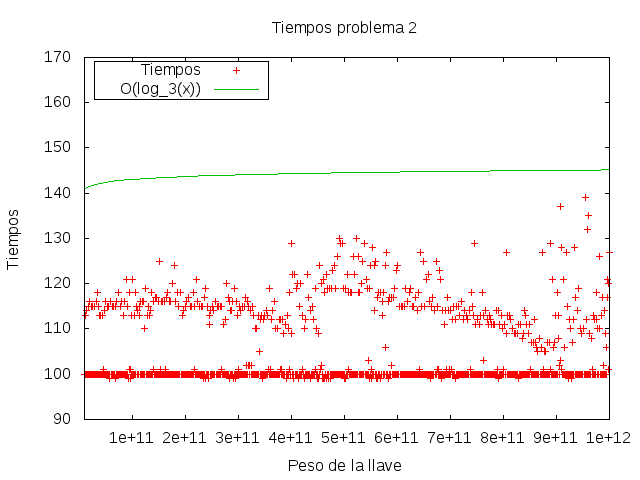
\includegraphics[width=15cm]{./imagenes/tiemposEj2.png}
    %\caption{FCFS con 2 núcleos}
    %\label{fig:my_label}
\end{figure}


En el siguiente gráfico se testearon pesos más grandes desde $10^{10}$ hasta $10^{12}$ y se ve que se cumple con la cota propuesta. Como puede observarse, la mayoría de los tiempos obtenidos en los experimentos tienen un valor similar a la experimentación anterior. Nuevamente esto se debe a que la diferencia entre tiempos al ser una complejidad logarítmica entre distintos tamaños de instancia es muy chica: en estas instancias con valores elevados la curva logarítmica es tan leve que al tomar sus valores enteros superiores se comporta como una recta constante en este rango de instancias.




\newpage

\section{Problema III: Guardando el tesoro}

\subsection{Introducción}

Una vez pasadas todas las pruebas, Indy y el grupo de arqueólogos se encuentran en una sala llena con N tipos de tesoros de los que se sabe su valor y su peso. 
El grupo desea saquear el templo maximizando el beneficio del botín que pueden meter en sus M mochilas de capacidades diferentes.
Para decidir que tipos de tesoros tomar y en que cantidad, se pidió desarrollar un algoritmo que devuelva el valor del mejor botín y como deben estar distribuidos los tesoros en las distintas mochilas.

En las próximas secciones se usarán las siguientes notaciones para referir a distintas variables del problema:

\begin{itemize}
\item $M =$ cantidad de mochilas disponibles
\item $N =$ cantidad de tipos de tesoros
\item $K_i = $ capacidad de la mochila $i$ ($1 \leq i \leq M$)
\item $C_i = $ cantidad de tesoros del tipo $i$ ($1 \leq i \leq N$)
\item $P_i = $ peso de cada tesoro $i$ ($1 \leq i \leq \sum C_i$)
\item $V_i = $ valor de cada tesoro del tipo $i$ ($1 \leq i \leq \sum C_i$)
\end{itemize}

\subsection{Resolución del problema}
La primer propuesta tomada en cuenta fue diseñar un algoritmo que haga uso de la técnica de backtracking para resolver problema. Sin embargo, la complejidad del mismo resultó ser $O(M*(\sum_{i=0}^{M}{C_i})!)$. Esto se debía a que, por las características de la técnica usada, se probaba poner toda las combinaciones posibles de tesoros en cada mochila.

Dicha complejidad superaba en demasía la complejidad pedida por el enunciado por lo que se estudiaron las propiedades del algoritmo para implementar la mayor cantidad de podas posibles e intentar, de esta forma reducir el tiempo de ejecución.

Durante esté análisis se vio que muchos casos, llegado a cierto punto, debían recalcular subproblemas que ya habían sido calculados en otro momento y se decidió cambiar el backtracking por el uso de programación dinámica para evitar este overhead innecesario.

\subsubsection{La función recursiva}
Suponiendo que los tesoros del templo están organizados en un array de longitud $\sum C_i$, en la que cada posición del mismo contiene un único tesoro (pudiendo haber repetidos si hay mas de un tesoro de un mismo tipo), se propuso la siguiente función recursiva para calcular cual es el mejor valor posible del botín:

\begin{align*}
F(i, x_1, \dots, x_n) = \mbox{Máximo valor posible del botín con } i \mbox{ tesoros y una mochila de capacidad } x_1, \\ \mbox{una de capacidad }x_2,\dots, \mbox{y una mochila de capacidad }x_n    
\end{align*}

Sea $F^j(i) = F(i, x_1,\dots,x_{j-1}, x_j - P_{i+1},x_{j+1}\dots,x_n)$ entonces se puede escribir $F$ como:
% TODO ARREGLAR
\begin{align*} 
F(i, x_1, \dots, x_n) =
\left\{
	\begin{array}{ll}
	    0 & \mbox{si } i = 0 \lor (\forall~ 1 \leq j \leq n) ~ x_i = 0 \\
	    F(i-1, x_1, \dots, x_n) & \mbox{si } (\forall~ 1 \leq j \leq n) ~ P_i > x_j \\
	    -\infty & \mbox{si } (\exists ~ 1 \leq j \leq n) ~x_i < 0 \\
	    max\left\{\begin{array}{c}
	        F(i-1, x_1, \dots, x_M), \\
	        V_i + F^1(i-1), \\
	        \vdots\\
	        V_i + F^j(i-1) \\
	        \vdots \\
	       V_i + F^n(i-1)\\
	    \end{array}
	       \right\} & \mbox{sino} \\
	\end{array}
\right.
\end{align*}

\newpage
La función está divida en 4 casos:
\begin{itemize}
\item  \textbf{Primer caso:} No hay tesoros que poner o todas las mochilas tienen capacidad cero. En este caso no hay botín posible y el mejor valor es $0$.
\item  \textbf{Segundo caso:} El $i$-ésimo tesoro no entra en ninguna de las mochilas disponibles, entonces se debe conseguir el mejor botín sin tenerlo en cuenta.
\item \textbf{Tercer caso:} Este es un caso especial al cual solo se llega si se intenta meter un tesoro cuyo peso es mayor a la capacidad de la mochila. En la función es tomado en cuenta para que en el cuarto caso, si sucede que una mochila no puede contener el tesoro el valor sea lo mínimo posible y no afecte al resultado real de la instancia del problema
\item \textbf{Cuarto caso:} El $i$-ésimo tesoro entra en una o más mochilas. Se busca maximizar el valor del botín, por lo tanto se calcula el máximo entre el valor del botín resultante de no poner el tesoro y el máximo botín conseguido al poner el tesoro en alguna mochila.
\end{itemize}

Se debe notar que en el último caso se calculan los valores del botín resultantes de poner el tesoro en cada mochila, cada uno de estos cálculos es necesario ya que las instancias más chicas generadas al meter el tesoro en mochilas distintas son distintas.

Por último, si se desea que la función devuelva la solución al problema propuesto se la debe llamar de la siguiente forma $F\left(\sum C_i, K_1, K_2,\dots,K_M\right)$

\subsubsection{Desarrollo del algoritmo}
Al momento de implementar la función se optó por resolverla con un algoritmo bottom-up que opere sobre los valores de una matriz multidimensional.

Dicha matriz, es una matriz de M + 1 dimensiones cuyos tamaños son las capacidades de las mochilas y la cantidad de tesoros incluidos en el botín. La celda $matriz[i_1,i_2,\dots,i_{M+1}]$ representa el valor $F(i_1, i_2,\dots,i_{M+1})$.

Se ve que la matriz generada es una matriz de $\left(\sum C_i\right)\times K_1\times\dots\times K_M$ celdas

De esta forma, todos las celdas cuyos índices son de la forma $[i, 0, 0,\dots,0]$ ó $[0, x_1, x_2, \dots, x_m]$ (que corresponden al caso base de la función) son inicializadas con ceros. A partir de aquí, la matriz se recorre de manera incremental calculando los valores de cada celda a partir de los valores de las celdas calculadas anteriormente. Para aclarar esto, el algoritmo resuelve el valor de la celda $[j,j_1,\dots,j_m]$ (que corresponde al valor $F(j,j_1,\dots,j_m)$) usando los valores de las celdas $[j-1,j_1,j_2\dots,j_m],[j-1,j_1,j_2-1,\dots,j_m],\dots,[j-1,j_1,j_2,\dots,j_{m-1}-1,j_m],[j-1,j_1,j_2-1,\dots,j_{m-1},j_m - 1]$ (es decir, de cada una de las celdas superiores respecto a cada una de sus dimensiones) de acuerdo a lo indicado por la función $F$.

Una vez calculados todos los valores, solo debemos encontrar el camino desde \\ $matriz\left[\sum C_i, K_1, K_2,\dots,K_M\right]$ hasta $matriz[0,K'_1,\dots,K'_2]$ que hace posible el valor guardado en la primer posición mencionada (los valores $K'_j$ son las capacidades finales de las mochilas, es posible que el mejor botín encontrado deje, en alguna de ellas, espacio que no pueda ser llenado por ninguno de los tesoros restantes).

Para encontrar este camino se usan los siguientes criterios:
\begin{itemize}
\item Si la mejor solución encontrada para el $i$-ésimo tesoro es igual a la mejor solución encontrada para el $(i-1)$-ésimo tesoro, entonces el $i$-ésimo tesoro no pertenece al botín.
\item Si lo primero no sucede, el tesoro pertenece al botín y debe ser puesto en algún mochila. Para identificar dicha mochila se debe probar meterlo en cada una de ellas hasta encontrar la celda cuyo valor sumado al valor del $i$-ésimo tesoro sea el valor del botín completo.
\end{itemize}

\newpage
\subsection{Pseudocódigo}

Todos los algoritmos tienen acceso a \textit{tesoros} la lista de tesoros y \textit{mochilas} la lista de mochilas disponibles.

\begin{algorithm}[H]
\caption{Resolver}
\begin{algorithmic}[1]
\Procedure{Resolver}{}

  	\State	dimensions $\gets\left[\sum C_i, K_1, \dots, K_M\right]$  \Comment O(M + 1)
	\State	matrix $\gets$ MultidimensionalMatrix(dimensions);	 \Comment O($\prod$ dimensions[i])
    \State  index $\gets$ [1,0,\dots,0]  \Comment Hay M ceros O(M+1)
    
    \While{index[0] $\leq$ $\sum C_i$} \Comment Se repite $\prod$ dimensions[i] veces
		\State	matrix.set(index, maxValue(matrix, index)) \Comment Setear la celda index de la  matriz al 
		\State  \Comment valor correspondiente O(M)
		\State	index $\gets$ nextIndex(matrix, index) \Comment O(1)
	\EndWhile
	\State	index $\gets$ previousIndex(matrix,index);
	\State	lootValue $\gets$ matrix.get(index);
	
	\While{index[0] $>$ 0}	 \Comment Se repite $\prod$ dimensions[i] veces
		\State	m $\gets$ whereToPutTreasure(matrix, index); \Comment Conseguir la mochila donde poner el tesoro O(m)
	    \If{m $<$ 0}
			\State	index[0] $\gets$ index[0] - 1; \Comment No poner el tesoro
        \Else	
			\State agregar(tesoros[index[0]], mochilas[m]) \Comment Agregar el tesoro a la $m$-ésima mochila. O(1)
			\State	index[0] $\gets$ index[0] - 1; \Comment Con estas dos líneas se mueve a la celda que representa
			\State	index[m] $\gets$ index[m] - peso(tesoros[index[0]]) \Comment la instancia generada al poner el 
			\State \Comment tesoro en la mochila
		\EndIf
    \EndWhile
\EndProcedure
\end{algorithmic}
\end{algorithm}

El paso en el que se rellenan con ceros las posiciones indicadas por el caso base de la función recursiva es omitido pues se asume que todas los valores de la matriz son inicializados en cero.

\begin{algorithm}[H]
\caption{maxValue}
\begin{algorithmic}
 
  \Procedure{maxValue}{MultidimensionalMatrix matrix, Integer[] index} $\to $ \texttt{Integer}
 		
 		\State auxIndex $\gets$ index
		\State auxIndex[0] $\gets$ auxIndex[0] - 1 \Comment Esta es la celda que corresponde a no poner el tesoro index[0]

        \State maxValue $\gets$ matrix.get(auxIndex) \Comment El valor del botín sin el tesoro
        \For {m = 1 to dimensiones(matrix)}  \Comment Se repite M veces
			\If{index[m] $>=$ peso(tesoros[index[0]])} \Comment Si la capacidad de la mochila $m$ es suficiente
			\State	auxIndex[m] $\gets$ index[m] - peso(tesoros[index[0]]); \Comment Poner el tesoro en la mochila $m$ O(1)
			\State	newValue $\gets$  valor(tesoro[index[0]]) + matrix.get(auxIndex); \Comment Conseguir el valor del botín \If{newValue $>$ maxValue} \Comment Si el valor que se consigue es mejor que el de los otros intentos
			\State maxValue $\gets$ newValue; \Comment se setea como maximo
			\EndIf
			
			\State auxIndex[m] $\gets$ auxIndex[m] + peso(tesoros[index[0]]) 	\Comment Sacar el tesoro de la mochila
			\EndIf
		\EndFor
    	\State Devuelvo maxValue
	\EndProcedure
 \end{algorithmic}
\end{algorithm}

\begin{algorithm}[H]
\caption{whereToPutTreasure}
\begin{algorithmic}[1]
  \Procedure{whereToPutTreasure}{MultidimensionalMatrix matrix, Integer[] index} $\to $ \texttt{Integer}

    \State auxIndex $\gets$ index 
    \State auxIndex[0] $\gets$ index[0]-1 
	\State actualValue $\gets$ matrix.get(index)
	\State maxValue $\gets$ matrix.get(auxIndex);
	
	\If{maxValue == actualValue}    \Comment Si el botín con el tesoro y el botín sin el tesoro
	    	\State Devolver -1  \Comment  tienen el mismo valor entonces omitirlo
	\EndIf
		
	\State	maxValue $\gets$ 0  \Comment Setear el valor maximo a cero

    \For {m = 1 to dimensiones(matrix)}  \Comment Se repite M veces
		\If{index[m] $\geq$ peso(tesoros[index[0]])} 
		\State	auxIndex[m] $\gets$ index[m] - peso(tesoros[index[0]])
		\State	newValue $\gets$  valor(tesoro[index[0]]) + matrix.get(auxIndex);

    	\If{newValue == actualValue)}	
            \State	whereToPut $\gets$ m 
            \State	maxValue $\gets$ newValue
		\EndIf
		\State	auxIndex[m] $\gets$ index[m] 
    \EndIf
	\EndFor
		
	\State	Devolver whereToPut
\EndProcedure
\end{algorithmic}
\end{algorithm}

Se puede ver que las funciones whereToPutTreasure y maxValues son similares. En ambas funciones se checkean los valores de las soluciones anteriores para decidir, en una, cual es el máximo valor de botín posible y, en la otra, en que mochila debo ubicar cierto tesoro para conseguir el botín que corresponde al valor ubicado en la celda pasada por parámetro.

\subsection{Correctitud}
El algoritmo propuesto puede ser dividido en partes:
\begin{enumerate}
    \item El cálculo del valor del mejor botín
    \item Calcular los tesoros que pertenecen a dicho botín y en que mochila deben ser guardados.
\end{enumerate}

Como se explicó en la sección 4.3.3, la primer parte del algoritmo corresponde al cálculo de la función $F$ para sus distintos parámetros de entrada.

\subsubsection{Primer parte}
Por inducción, se puede ver que el primer paso es correcto:

\textbf{Casos Base:}

\begin{itemize}
\item $\sum C_i = 0$:
    
    Al no haber tesoros que poner en las mochilas, no hay botín posible, por lo tanto no hay valor positivo para el mismo.
    
    En la implementación del algoritmo, la matriz es inicializada con todos sus valores en $0$ pero no es modificada por el while correspondiente a esta parte del algoritmo. Por lo que $lootValue = 0$.
    
\item $K_i = 0 ~\forall~ 1\leq i \leq M$

    Todas las mochilas tienen capacidad cero y como el peso de cualquier tesoro es mayor a cero, entonces no existe un tesoro que entre en ninguna de ellas. Esto quiere decir que no hay botín posible, entonces, no hay valor positivo para el mismo.
    
    Otra vez, se ve que el algoritmo respeta este caso, las iteraciones son realizadas, pero al momento de calcular el máximo valor del botín, se toma el valor de la solución anterior (que es 0) y se itera sobre todas las mochilas. Sin embargo, al tener todas ellas capacidad cero, en ninguna iteración se accede al if que remplaza el valor máximo por uno distinto. Luego, el resultado de esta operación termina siendo cero.
    
    En un primer paso se calcula el valor de poner cero tesoros en las mochilas (este es el caso anterior) entonces este valor es cero. Luego, se trata de poner un tesoro pero, por las operaciones que realiza el algoritmo este valor será el mismo que el de la solución anterior entonces el mejor botín con un tesoro tiene valor 0.
    
    En el n-ésimo paso, la solución será la misma que en el (n-1)-ésimo que, como se explicó, es 0. Esto implicaría que en el n-ésimo paso la solución seguirá siendo 0.
    
    Por último, habiendo demostrado esto, se concluye que en último valor calculado \\ $\left(M\left[\sum C_i, K_1, \dots, K_M\right]\right)$ es 0.
\end{itemize}

\textbf{Paso inductivo:}

    Sea la hipótesis inductiva que el algoritmo es correcto para todas las instancias tal que hay $i-1$ tesoros, se puede deducir la correctitud del $i$-ésimo:
    
    \begin{align*}
    F(i, x_1,\dots,x_M) &= 	max\left\{ F(i-1, x_1, \dots, x_M), V_i + F^1(i-1), \dots,
	        V_i + F^j(i-1), \dots, V_i + F^n(i-1)\right\} \\ &= max\left\{F(i-1, x_1,
	        \dots, x_M), V_i + max\left\{F^1(i-1), \dots, F^j(i-1), \dots, F^n(i-1)\right\}\right\}    
    \end{align*}
    
    Por la hipótesis inductiva, sabemos que $ F(i-1, x_1, \dots, x_M)$, $F^1(i-1),\dots, F^n(i-1)$ son correctas.
    
    Se puede ver que la función toma el máximo entre todas las posibilidades dados $i$ tesoros con la configuración de mochilas dadas.
    
    La función devuelve el máximo valor de entre no agregar el tesoro y agregarlo a alguna mochila. Por \textit{HI}, el primer valor es correcto, veamos que el segundo valor lo es:
    
    El segundo valor toma el máximo botín que se puede obtener si fuese que se reserva un lugar para el $i$ ésimo tesoro en alguna mochila.
    Si $F^j(i-1)$ corresponde al mejor botín posible con esta característica, entonces el segundo valor es de la forma $V_i + F^j(i-1)$. Y si este no fuera el mejor valor posible, entonces existiría otro botin con valor $V_i + F^k(i-1)$, en este caso resultaria que $F^k(i-1) > F^j(i-1)$ pero esto sería absurdo por que $F^j(i-1)$ era el máximo.
    
    El algoritmo propuesto realiza esta operación de la manera clásica, asigna un valor inicial a la variable $maxValue$ ($ F(i-1, x_1, \dots, x_M)$) y luego itera sobre las posiciones de la matriz que corresponden a intentar meter el botín en las distintas mochilas disponibles. Cuando se ve que, al ubicar el tesoro en cierta mochila, se consigue un valor mayor a $maxValue$, este es reemplazado por el nuevo valor encontrado.
    
    Al finalizar las iteraciones, $maxValue$ contendrá el máximo valor posible del botín.
    
\subsubsection{Segunda parte}
Este paso consiste en reproducir las selecciones de los máximos elegidos en la sección anterior. Para esto, se checkean uno a uno los valores de cada instancia más chica del problema llamada en $F$.

La primer celda checkeada corresponde a la solución en la que el tesoro no es agregado y si el valor de esta solución y la solución que se esta buscando es igual, entonces el tesoro es omitido.
Al resto de los valores se le suma el valor del tesoro que se intenta agregar, si el resultado es igual al valor de la celda que se está analizando entonces el tesoro se agrega a la mochila que corresponde al índice desplazado. 
Este desplazamiento corresponde al valor máximo elegido por la función $F$ y estas operaciones se realizan de forma iterativa hasta que la celda analizada represente alguno de los casos bases de $F$.

Cuando el algoritmo finaliza, las mochilas contienen la sucesión de tesoros necesaria para poder lograr un botín de valor óptimo.

\subsection{Complejidad del algoritmo}

Al momento de calcular la complejidad de los algoritmos propuestos se asumió que el acceso a una posición de la matriz multidimensional es $O(1)$. 

\subsubsection{maxValue y whereToPut}
En los algoritmos $maxValue$ y $whereToPutTreasure$, los $for$ realizan $M$ iteraciones en las cuales se accede y/o modifica la matriz y distintas variables enteras, cada una de estas operaciones es $O(1)$. En ambos casos los condicionales de los $if$ dentro del $for$ hacen comparaciones de enteros por lo que estas comparaciones se realizan en $O(1)$.
Las asignaciones realizadas fuera del $for$ son realizadas en $O(1)$, salvo la variable $auxIndex$ que es inicializada en $O(M+1)$.

Luego ambos algoritmos son de complejidad $O(M + M + 1) \subset O(M)$.

\subsubsection{resolver}
En el algoritmo $resolver$, se crean 2 arrays (\texttt{dimensions} e \texttt{index}) de $M+1$ elementos cada uno ($O(M+1)$), luego se crea la matriz multidimensional que es $O\left(\prod\texttt{dimensions}[i]\right)$ y luego se ejecutan los dos $while$. 

Con el primer $while$ se rellena cada posición de la matriz con el valor correspondiente, esto es hacer $\prod\texttt{dimensions}[i]$ iteraciones. En cada iteración se debe setear la celda correspondiente usando la función $maxValue$ ($O(M)$) y luego se aumenta el indice en 1 ($O(1)$). Entonces el $while$ completo tiene complejidad $O\left(M*\prod\texttt{dimensions}[i]\right)$

En el segundo, en peor caso, debemos volver a recorrer cada celda de la matriz por lo que se realizan la misma cantidad de iteraciones. En cada iteración se realiza una llamada a $whereToPut$ ($O(M)$) y a luego se calcula el proximo indice en $O(1)$, además, si es necesario, se agrega a una mochila un tesoro.

Las mochilas pueden ser vistas como listas enlazadas, por lo que agregarles un elemento es $O(1)$.

Por lo tanto el segundo while tiene la misma complejidad que el primero.

El algoritmo completo tiene complejidad 

$$O\left(M + 1 + M*\prod\texttt{dimensions}[i] + M*\prod\texttt{dimensions}[i]\right) \subset O\left(M*\prod\texttt{dimensions}[i]\right)$$

Ahora, \texttt{dimension[0]} es la cantidad de tesoros en la sala, es decir $\sum_{i=1}^N C_i$, entonces:

$$ M*\prod_{i=0}^M\texttt{dimensions}[i] = M*\left(\sum_{i=1}^N C_i\right)*\prod_{i=1}^M\texttt{dimensions}[i]$$

Y cada uno de los indices siguientes, corresponden a los pesos de los mochilas, es decir $indice[i] = K_i$ para $1 \leq i \leq M$ y vale:

$$M*\left(\sum C_i\right)*\prod_{i=1}^M\texttt{dimensions}[i] = M*\left(\sum C_i\right)*\prod_{i=1}^M K_i$$

Luego el algoritmo completo es de complejidad $O(M*\left(\sum_{i=1}^N C_i\right)*\prod_{i=1}^M K_i)$, solo falta ver que dicha complejidad es menor a la requerida por el enunciado, es decir se necesita comprobar que:


\[
O\left(M*\left(\prod_{i=1}^{M}{K_i}\right)*\left(\sum_{i=1}^{N}{C_i}\right)\right) \subset O\left(\left(\sum_{i=1}^{M}{K_i}\right)^{M}*\left(\sum_{i=1}^{N}{C_i}\right)\right)
\]

Para ver que esto es cierto basta con probar la siguiente desigualdad:

\[
M*\left(\prod_{i=1}^{M}{K_i}\right)*\left(\sum_{i=1}^{M}{C_i}\right) \leq \left(\sum_{i=1}^{M}{K_i}\right)^{M}*\left(\sum_{i=1}^{N}{C_i}\right)
\]

Como $\sum_{i=1}^{N}{C_i} \neq 0$ :

\[
M*\prod_{i=1}^{M}{K_i} \leq \left(\sum_{i=1}^{N}{K_i}\right)^{M}
\]

Por la fórmiula del coeficiente multinomial se sabe que:

\begin{align*}
\left(\sum_{i=1}^{M}{K_i}\right)^{M} =  \sum_{J_1+...+J_M=M}\binom{M}{ J_1,...,J_M}*\prod_{t=1}^{M}{K_i}^{J_t} = \\
M * \prod_{i=1}^M K_i + 
\sum_{ J_1,\dots,J_M : J_1 + \dots + J_M = M \land  \lnot (\forall 1 \leq i \leq M) J_i = 1}\binom{M}{ J_1,...,J_M}*\prod_{t=1}^{M}{K_i}^{J_t}
\end{align*}

El primer término mostrado en la última igualdad surge de elegir todos los exponentes iguales a 1. Por esta razón se agrega la condición $\lnot (\forall 1 \leq i \leq M) J_i = 1$ al segundo término.

En la inecuación, entonces se remplaza:

\[
M*\left(\prod_{i=1}^{M}{K_i}\right) \leq M * \prod_{i=1}^M K_i + 
\sum_{ J_1,\dots,J_M : J_1 + \dots + J_M = M \land  \lnot (\forall 1 \leq i \leq M) J_i = 1}\binom{M}{ J_1,...,J_M}*\prod_{t=1}^{M}{K_i}^{J_t}
\]

\[
0\leq \sum_{ J_1,\dots,J_M : J_1 + \dots + J_M = M \land  \lnot (\forall 1 \leq i \leq M) J_i = 1}\binom{M}{ J_1,...,J_M}*\prod_{t=1}^{M}{K_i}^{J_t}
\]


Y como todos los elementos de esta sumatoria son enteros positivos (por ser todos los $K_i$ positivos), queda demostrado que la complejidad que proponemos es menor a la pedida por el enunciado.

\subsection{Experimentación}
Para los experimentos se decidió analizar instancias se varían los tamaños de las mochilas y la cantidad de tesoros por separado. En ambos experimentos, las variaciones se prueban para 1, 2 y 3 mochilas.

En el primero de los casos, se fijó el tamaño de las mochilas en 50 unidades cada una y se generaron instancias de problemas con cantidades de tesoros variante entre 1 y 100. El precio y valor de cada uno de los tesoros fue generado aleatoriamente entre los valores 1 y 100.

Se debe notar que los valores y pesos de los tesoros no influyen en la complejidad del algoritmo por lo que no se consideró necesario evaluar instancias con valores demasiados granes.

Los resultados obtenidos se muestran en los siguiente gráficos:
\begin{figure}[H]
    \centering
    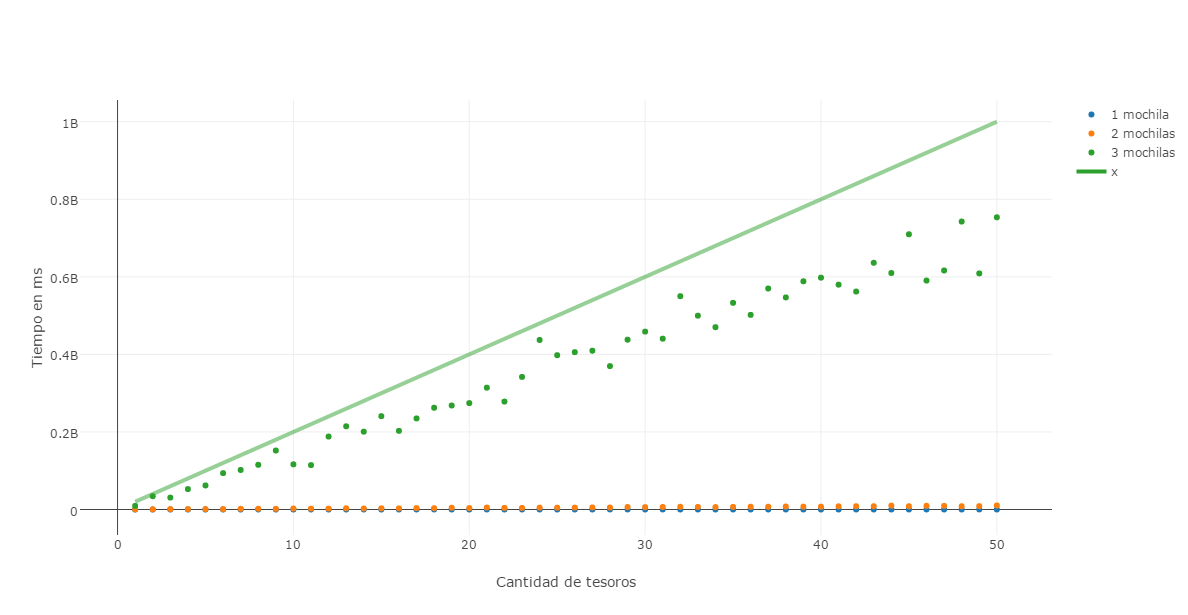
\includegraphics[width=\textwidth]{./imagenes/3-1.png}
\end{figure}

Se puede ver que para los 3 casos probados el crecimiento temporal es lineal, lo que corresponde con la complejidad teórica calculada cuando la cantidad de mochilas y sus capacidades son tomadas como constantes. Y además, se nota que al aumentar la cantidad de mochilas los tiempos para instancias con la misma cantidad de tesoros incrementan notablemente debido a que la constante se ve afectada exponencialmente por la cantidad de mochilas.

$$O\left(\left(\sum_{i=1}^{1}{50}\right)^{1}*\left(\sum_{i=1}^{N}{C_i}\right)\right) = O\left(\sum_{i=1}^{N}{C_i}\right) = 
O\left(X\right)$$


$$
O\left(\left(\sum_{i=1}^{2}{50}\right)^{2}*\left(\sum_{i=1}^{N}{C_i}\right)\right) = O\left(\sum_{i=1}^{N}{C_i}\right) = O\left(X\right)$$

$$O\left(\left(\sum_{i=1}^{3}{50}\right)^{3}*\left(\sum_{i=1}^{N}{C_i}\right)\right) = O\left(\sum_{i=1}^{N}{C_i}\right) = O\left(X\right)$$

En el siguiente, se ha realizado un experimento similar anterior diferenciándose de que todas las instancias los tesoros van a ser los mismos y se varían las capacidades de las mochilas. 

Los tesoros elegidos fueron:

\begin{tabular}{ c c c }
    Cantidad & Peso & Valor \\
    1 & 30 & 14 \\
    3 & 35 & 10 \\
    4 & 40 & 30 \\
    2 & 45 & 4 \\
    1 & 50 & 20 \\
    5 & 50 & 60 \\
\end{tabular}
 
						

En este caso, el polinomio que acota temporalmente a los tiempos calculados está dado por la cantidad de mochilas. En el siguiente gráfico se observa que para 1 mochila, los tiempos se incrementan de forma lineal, mientras que en las instancias de 2 mochilas su aumento es cuadrático y en las de 3 mochilas es cúbico.

\begin{figure}[H]
    \centering
    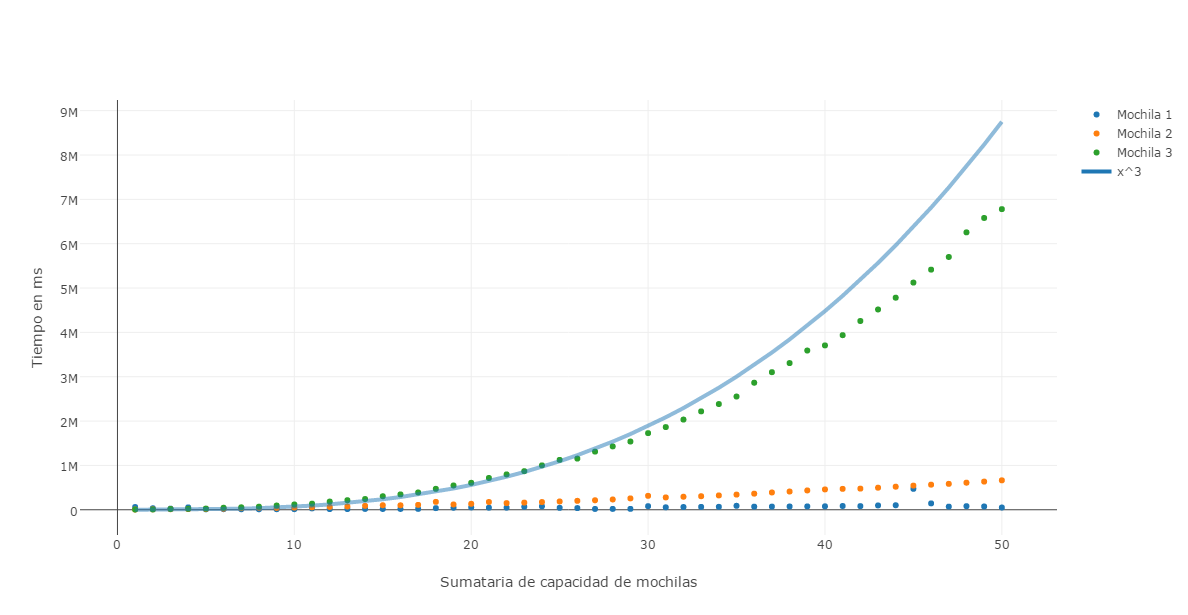
\includegraphics[width=\textwidth]{./imagenes/3-2.png}

\end{figure}

De esta forma se corrobora que la complejidad se cumpla, ya que la complejidad experimental de cada caso termina siendo:
Sea $K_i$ al peso de la i-ésima mochila:

$$O\left(\left(\sum_{i=1}^{1}{K_i}\right)^{1}*\left(\sum_{i=1}^{6}{C_i}\right)\right) = O\left(\left(\sum_{i=1}^{1}{K_i}\right)^{1}*\left(16\right)\right) = O\left(K_1\right)$$

$$O\left(\left(\sum_{i=1}^{2}{K_i}\right)^{2}*\left(\sum_{i=1}^{6}{C_i}\right)\right) = O\left(\left(\sum_{i=1}^{2}{K_i}\right)^{2}*16\right) = O\left(\left(\sum_{i=1}^{2}{K_i}\right)^{2}\right)$$

$$O\left(\left(\sum_{i=1}^{3}{K_i}\right)^{3}*\left(\sum_{i=1}^{6}{C_i}\right)\right) = O\left(\left(\sum_{i=1}^{3}{K_i}\right)^{3}*16\right) = O\left(\left(\sum_{i=1}^{3}{K_i}\right)^{3}\right) $$

\newpage

\section{Hoja de cambios:}

\subsection{Problema 1}

\begin{itemize}

\item En la tabla de ejemplos de la sección 2.1.1 se cambió el nombre de Puente por Movimiento, para diferenciar más el puente del problema original con el objeto Puente

\item Se mejoraron los textos de Resolución del problema, Algoritmos y Complejidad.

\item Se agregó el algoritmo $enviarArq$ y se expandió el pseudocódigo de $prueboEnviar2Arqueologos$ para mayor claridad.

\item Se explicó el cambio en la complejidad de algunos algoritmos, que en el cálculo se tiene en cuenta la recursión pero para otras operaciones no.

\item Se dio una mejor explicación de porqué el programa termina y una demostración de porqué el algoritmo recorre todos los estados válidos.

\item Se explicó porqué la altura máxima del árbol es de $\mathcal{O}((N+M)!)$

\item Se agregó la descripción del generador de casos aleatorios para graficar los tiempos del algoritmo. Además, se agregó un gráfico fijando N en un caso y M en el otro.

\end{itemize}

\subsection{Problema 2}

\begin{itemize}

    \item Se corrigió la demostración de la complejidad.
    
    \item Se explicó de mejor manera los resultados obtenidos en la experimentación realizada.

\end{itemize}

\subsection{Problema 3}

\begin{itemize}
\item Se explicó de mejor manera función recursiva
\item Se cambió el paso inductivo de la demostración de correctitud para que sea más entendible.
\end{itemize}

\end{document}
